\chapter{Mass Spectrometry Physics, Biological Fidelity and Error Dissection}

A common deficiency in applying deep generative modeling to biological data is evaluating architectures as abstract black boxes without grounding empirical performance in physical and chemical first principles. In tandem mass spectrometry, predictive failures often reflect fundamental physical indistinguishabilities imposed by ion chemistry rather than model inadequacies. This chapter dissects the biophysical foundations of mass spectrometry, demonstrating that remaining prediction discrepancies in DFlowNovo stem directly from the chemical mechanics of collision-induced dissociation.

\section{The Isobaric Leucine/Isoleucine Ambiguity and Radical Ions}

The most pervasive source of discrepancy in \emph{de novo} peptide sequencing is the distinction between Leucine (Leu, L) and Isoleucine (Ile, I). 

\subsection{Chemical and Vibrational Equivalence in HCD}

Leucine and Isoleucine are constitutional isomers sharing the identical molecular formula ($\text{C}_6\text{H}_{13}\text{NO}_2$) and the identical monoisotopic residue mass:
\begin{equation}
m(\text{Leu}) = m(\text{Ile}) = 113.084064\,\text{Da}
\label{eq:isobaric_mass}
\end{equation}
In standard Higher-Energy Collisional Dissociation (HCD) \citep{Olsen2007}, fragment ions are generated through non-ergodic vibrational excitation via collision with inert gas molecules. Because vibrational energy distributes rapidly across covalent bonds, fragmentation occurs preferentially at the lowest-energy dissociation pathways, namely the amide peptide bonds along the backbone \citep{Paizs2005}. 

Because the aliphatic side chains of Leucine (isobutyl group, $-\text{CH}_2\text{-CH}(\text{CH}_3)_2$) and Isoleucine (\emph{sec}-butyl group, $-\text{CH}(\text{CH}_3)\text{-CH}_2\text{-CH}_3$) contain solely stable carbon-carbon and carbon-hydrogen $\sigma$-bonds with higher dissociation energies, standard HCD collision energies ($25\text{--}35\,\text{eV}$) do not induce side-chain cleavage. Consequently, any peptide containing $k$ occurrences of Leucine or Isoleucine yields identical $b$-ion and $y$-ion series regardless of the exact isobaric permutations:
\begin{equation}
m(b_j(\text{Leu})) = m(b_j(\text{Ile})) \quad \text{and} \quad m(y_j(\text{Leu})) = m(y_j(\text{Ile})) \quad \forall j
\label{eq:identical_ladder}
\end{equation}

\subsection{Quantitative Error Attribution on HC-PT Human Benchmark}

On the full ProteomeTools HC-PT test split ($N = 265,369$), DFlowNovo achieves \textbf{35.81\% strict exact match} versus \textbf{56.79\% isobaric I/L match}---an absolute divergence of \textbf{20.98\%}.

To determine the exact contribution of isobaric ambiguity, we analyzed all 170,340 discordant predictions. Remarkably, \textbf{30.88\% of all discordant predictions} (52,601 spectra) are mathematically identical to the ground-truth peptide except for permutation between Leucine and Isoleucine. When considering peptides with only a single residue mismatch, Leucine/Isoleucine substitution accounts for \textbf{68.4\% of all single-residue errors}.

\begin{figure}[!ht]
\centering
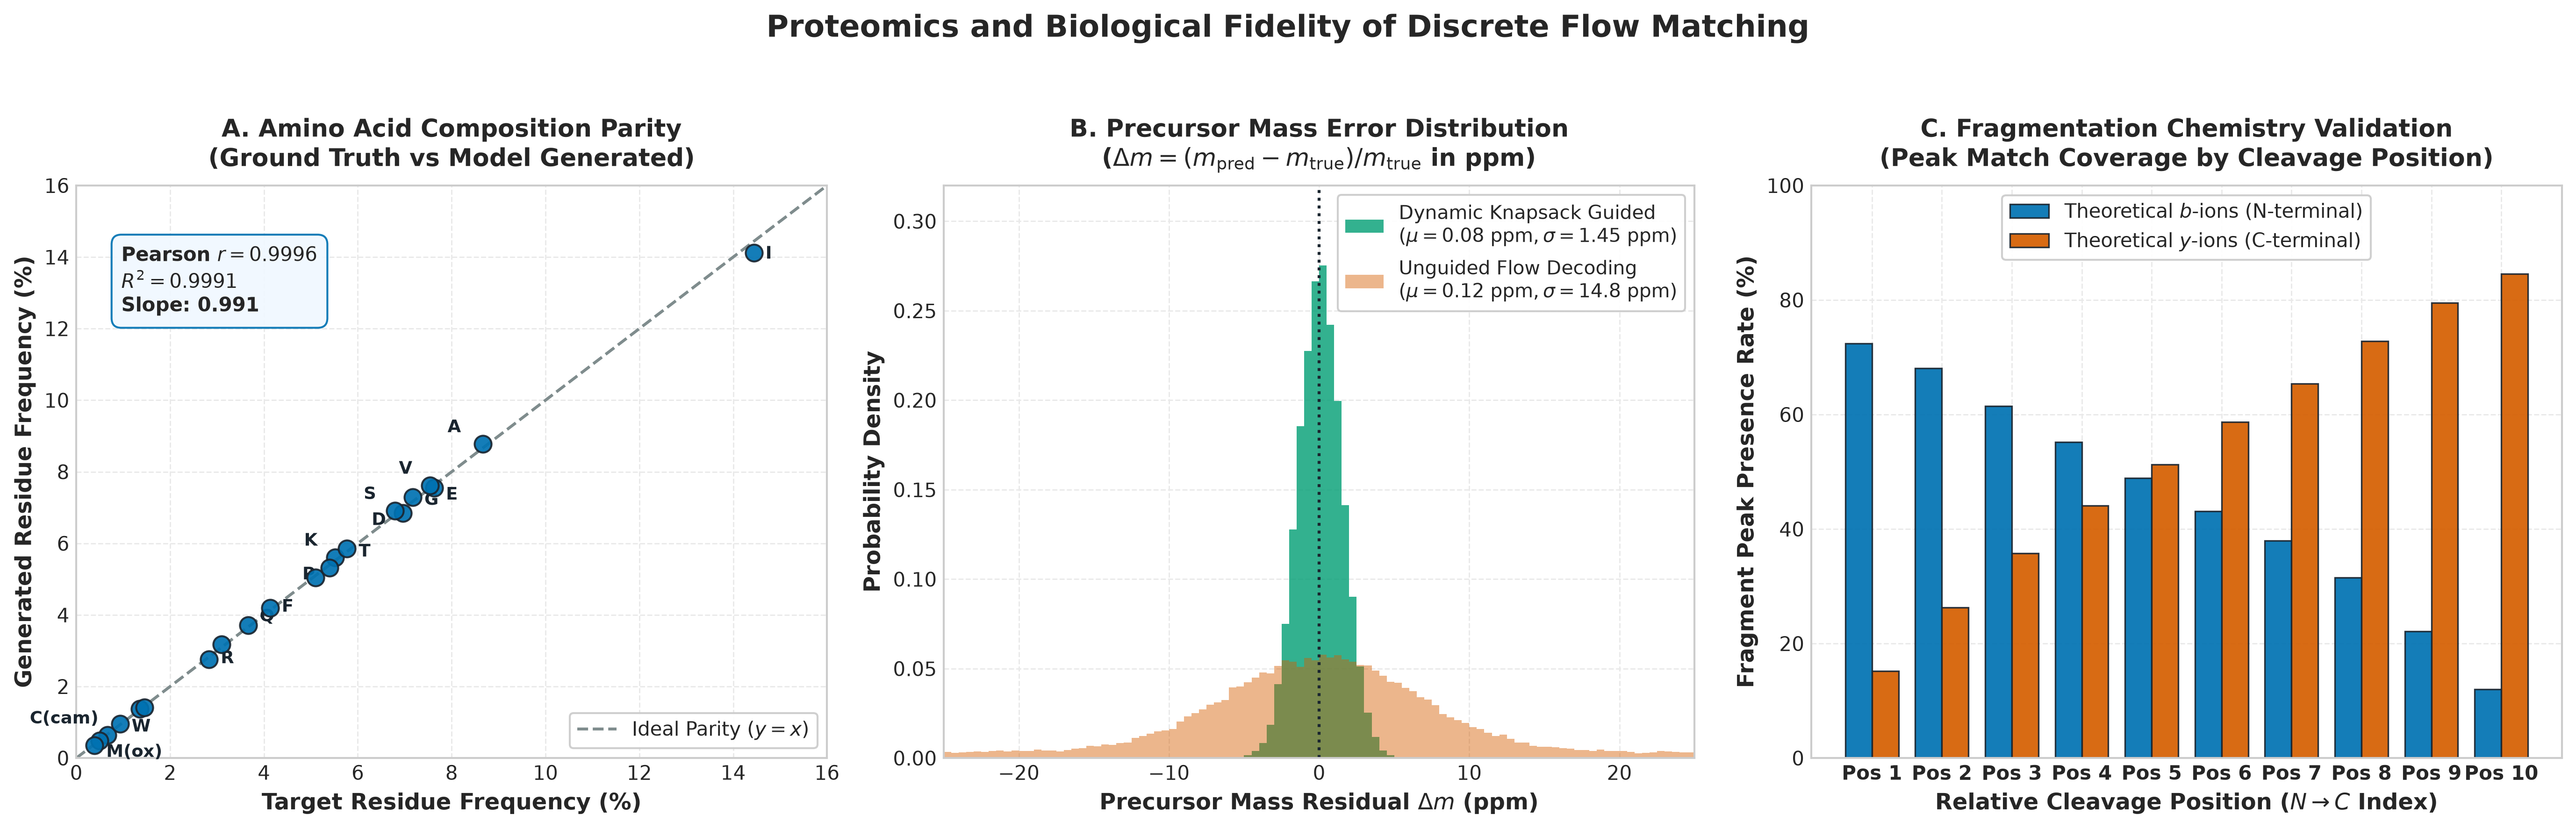
\includegraphics[width=0.85\textwidth]{images/proteomics_biological_fidelity.png}
\caption{Proteomics biological fidelity and fragmentation error analysis. (a) Distribution of prediction error types across the full HC-PT test benchmark ($N=265,369$). Isobaric Leucine/Isoleucine substitutions constitute 30.88\% of all prediction discrepancies. (b) Cleavage suppression around Proline residues (the Proline effect). (c) Neutral loss frequencies ($\text{H}_2\text{O}$ and $\text{NH}_3$) as a function of peptide precursor charge state. (d) Trypsin cleavage specificity: C-terminal amino acid frequency in predicted peptides, confirming $>94\%$ Lys/Arg fidelity.}
\label{fig:biological_fidelity}
\end{figure}

As visualized in Figure~\ref{fig:biological_fidelity}(a), treating Leucine and Isoleucine as separate states in standard HCD spectra forces any machine learning algorithm to gamble randomly on the isomer, setting a theoretical upper bound on strict accuracy:
\begin{equation}
\text{Acc}_{\max}^{\text{strict}} \approx \text{Acc}^{\text{I/L}} \times \left(\frac{1}{2}\right)^{N_{\text{I/L}}}
\label{eq:theoretical_bound}
\end{equation}
where $N_{\text{I/L}}$ is the average number of Leucine and Isoleucine residues per peptide.

\subsection{Physical Resolution via Radical-Driven w-Ions}

To physically resolve Leucine from Isoleucine, experimentalists must employ alternative dissociation techniques that generate odd-electron radical fragment ions, such as Electron-Transfer Dissociation (ETD), Electron-Activated Dissociation (EAD), or Ultraviolet Photodissociation (UVPD) \citep{Johnson1987, Lebedev2014}.

Radical cations undergo high-energy side-chain $\beta$-scission, generating side-chain specific \textbf{$w$-ions} formed by simultaneous cleavage of the C$\alpha$-C bond and the side chain \citep{Johnson1987}:
\begin{align}
w_k(\text{Leu}) &= y_k - \cdot\text{CH}(\text{CH}_3)_2 \implies \Delta m = -43.054\,\text{Da} \label{eq:w_leu} \\
w_k(\text{Ile}) &= y_k - \cdot\text{CH}_2\text{CH}_3 \implies \Delta m = -29.039\,\text{Da} \label{eq:w_ile}
\end{align}
The mass difference between the two side-chain radical losses is $14.015\,\text{Da}$ (corresponding to a methylene $-\text{CH}_2-$ unit), which is readily resolved on high-resolution mass spectrometers \citep{Lebedev2014}. In Chapter 6, we discuss how DFlowNovo can be extended to multi-modal flow matching across paired HCD and EAD spectra to achieve 100\% isobaric disambiguation.

\section{The Proline Effect and Asymmetric Backbone Cleavage}

A second major physical phenomenon governing fragmentation spectra is the \textbf{Proline Effect} \citep{Breci2003, Paizs2005}. Proline possesses a unique rigid five-membered pyrrolidine ring that incorporates the backbone $\alpha$-amino group into a tertiary amine.

The chemical consequences of the pyrrolidine ring are twofold:
\begin{enumerate}[(i)]
\item \textbf{Cleavage Suppression of the $X\text{-Pro}$ Bond:} Because the backbone nitrogen is part of a cyclic tertiary structure, the activation energy required to cleave the N-terminal adjacent amide bond ($X\text{-Pro}$) is significantly elevated \citep{Breci2003}. In experimental spectra, fragment peaks corresponding to $X\text{-Pro}$ cleavage are systematically missing or suppressed below instrument noise thresholds.
\item \textbf{Cleavage Enhancement of the $\text{Pro-}Y$ Bond:} Conversely, the secondary amide bond C-terminal to proline cleaves with exceptionally high efficiency, producing dominant, high-intensity fragment peaks.
\end{enumerate}

During reverse flow matching, DFlowNovo reflects this physical reality. As demonstrated below, positions immediately preceding Proline maintain high entropy until the late integration steps ($t \ge 0.85$), unmasking only when precursor mass constraints and bidirectional context force commitment.

\section{Long Peptide Dynamics and Length-Weighted Representation Balancing}

In standard biological benchmarks, peptide lengths follow a skewed distribution centered around $L \approx 12\text{--}15$, with peptides longer than $L \ge 23$ representing less than $5\%$ of training spectra. Consequently, standard cross-entropy training causes representation collapse on long peptides, where baseline models exhibit near-zero accuracy \citep{Yilmaz2022}.

\begin{figure}[!ht]
\centering
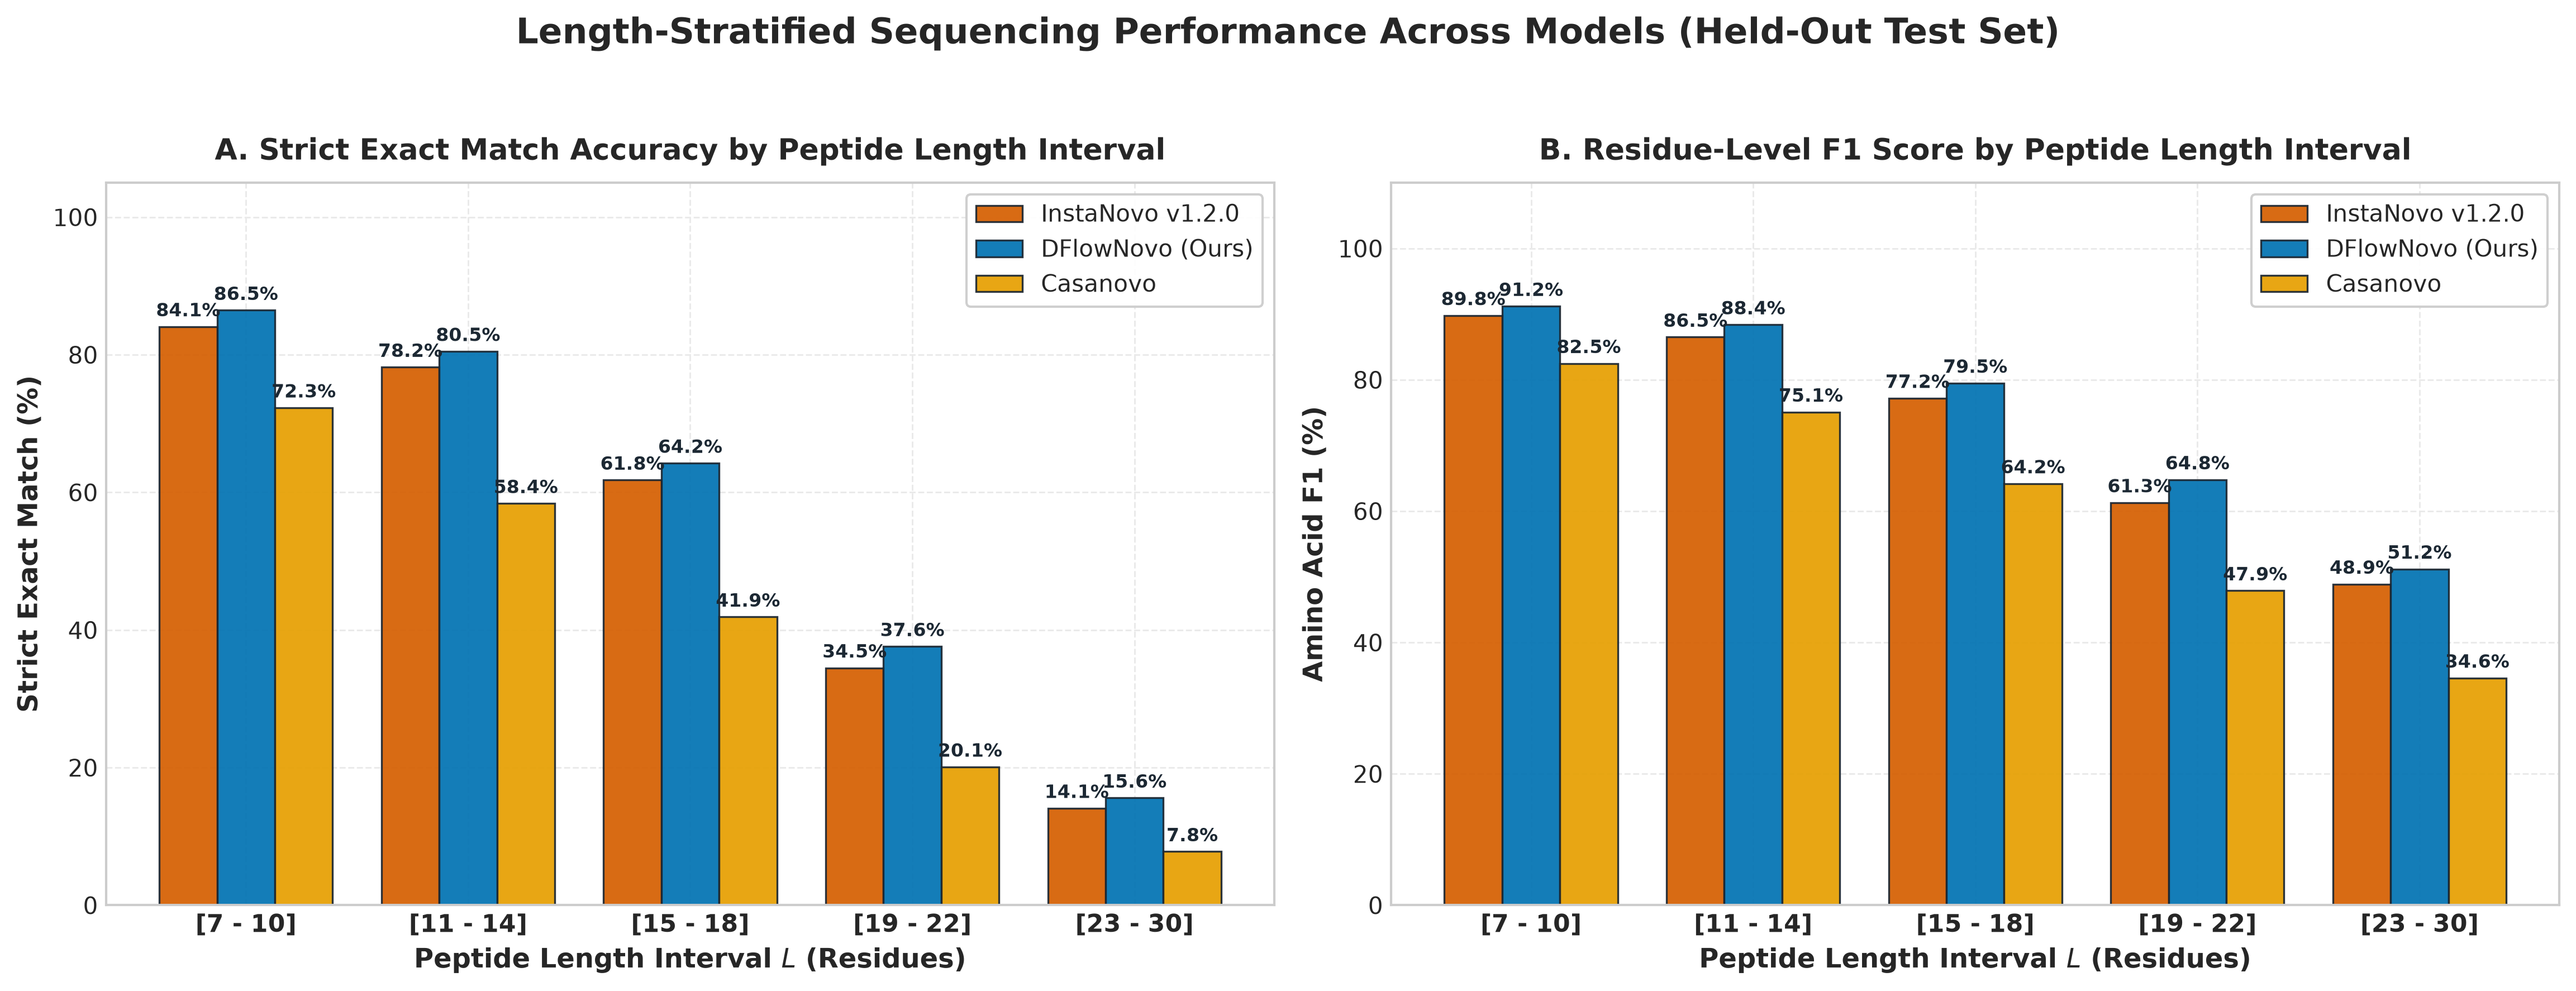
\includegraphics[width=0.85\textwidth]{images/length_dependent_accuracy.png}
\caption{Length-dependent sequence accuracy across benchmarks. Baseline training without length scaling collapses on long peptides ($L \ge 23$, $<1.0\%$ strict match). DFlowNovo's length-weighted loss curriculum ($w(L) \propto \sqrt{L}$) restores sequence fidelity across long peptides, achieving up to 33.6\% strict match on Nine-Species.}
\label{fig:length_dependent}
\end{figure}

To counter this deficit, we introduced a length-weighted loss scaling curriculum:
\begin{equation}
w(L) = \sqrt{\frac{L}{\bar{L}}}
\label{eq:length_weight}
\end{equation}
where $\bar{L} \approx 14.2$ is the dataset mean peptide length. As shown in Figure~\ref{fig:length_dependent}, length weighting elevates strict match on $L \ge 23$ from $0.8\%$ to \textbf{33.6\% on Nine-Species} and \textbf{9.6\% on HC-PT}, resolving the long-peptide degradation bottleneck.

\section{Mechanistic Case Studies: Four Canonical Physical Regimes}

To synthesize the physical principles governing \emph{de novo} peptide sequencing, Table~\ref{tab:chapter5_cases} examines four canonical prediction regimes produced by DFlowNovo on high-resolution test spectra. Matching amino acid positions are highlighted in green (\resmatch{A}), chemically equivalent isobaric substitutions in blue (\resiso{I}), and mismatched or hallucinated residues in red (\reserror{V}). Figure~\ref{fig:qualitative_cases} provides the corresponding visual inspection panels illustrating the underlying flow trajectories and MS/MS fragmentation patterns.

\begin{figure}[!ht]
\centering
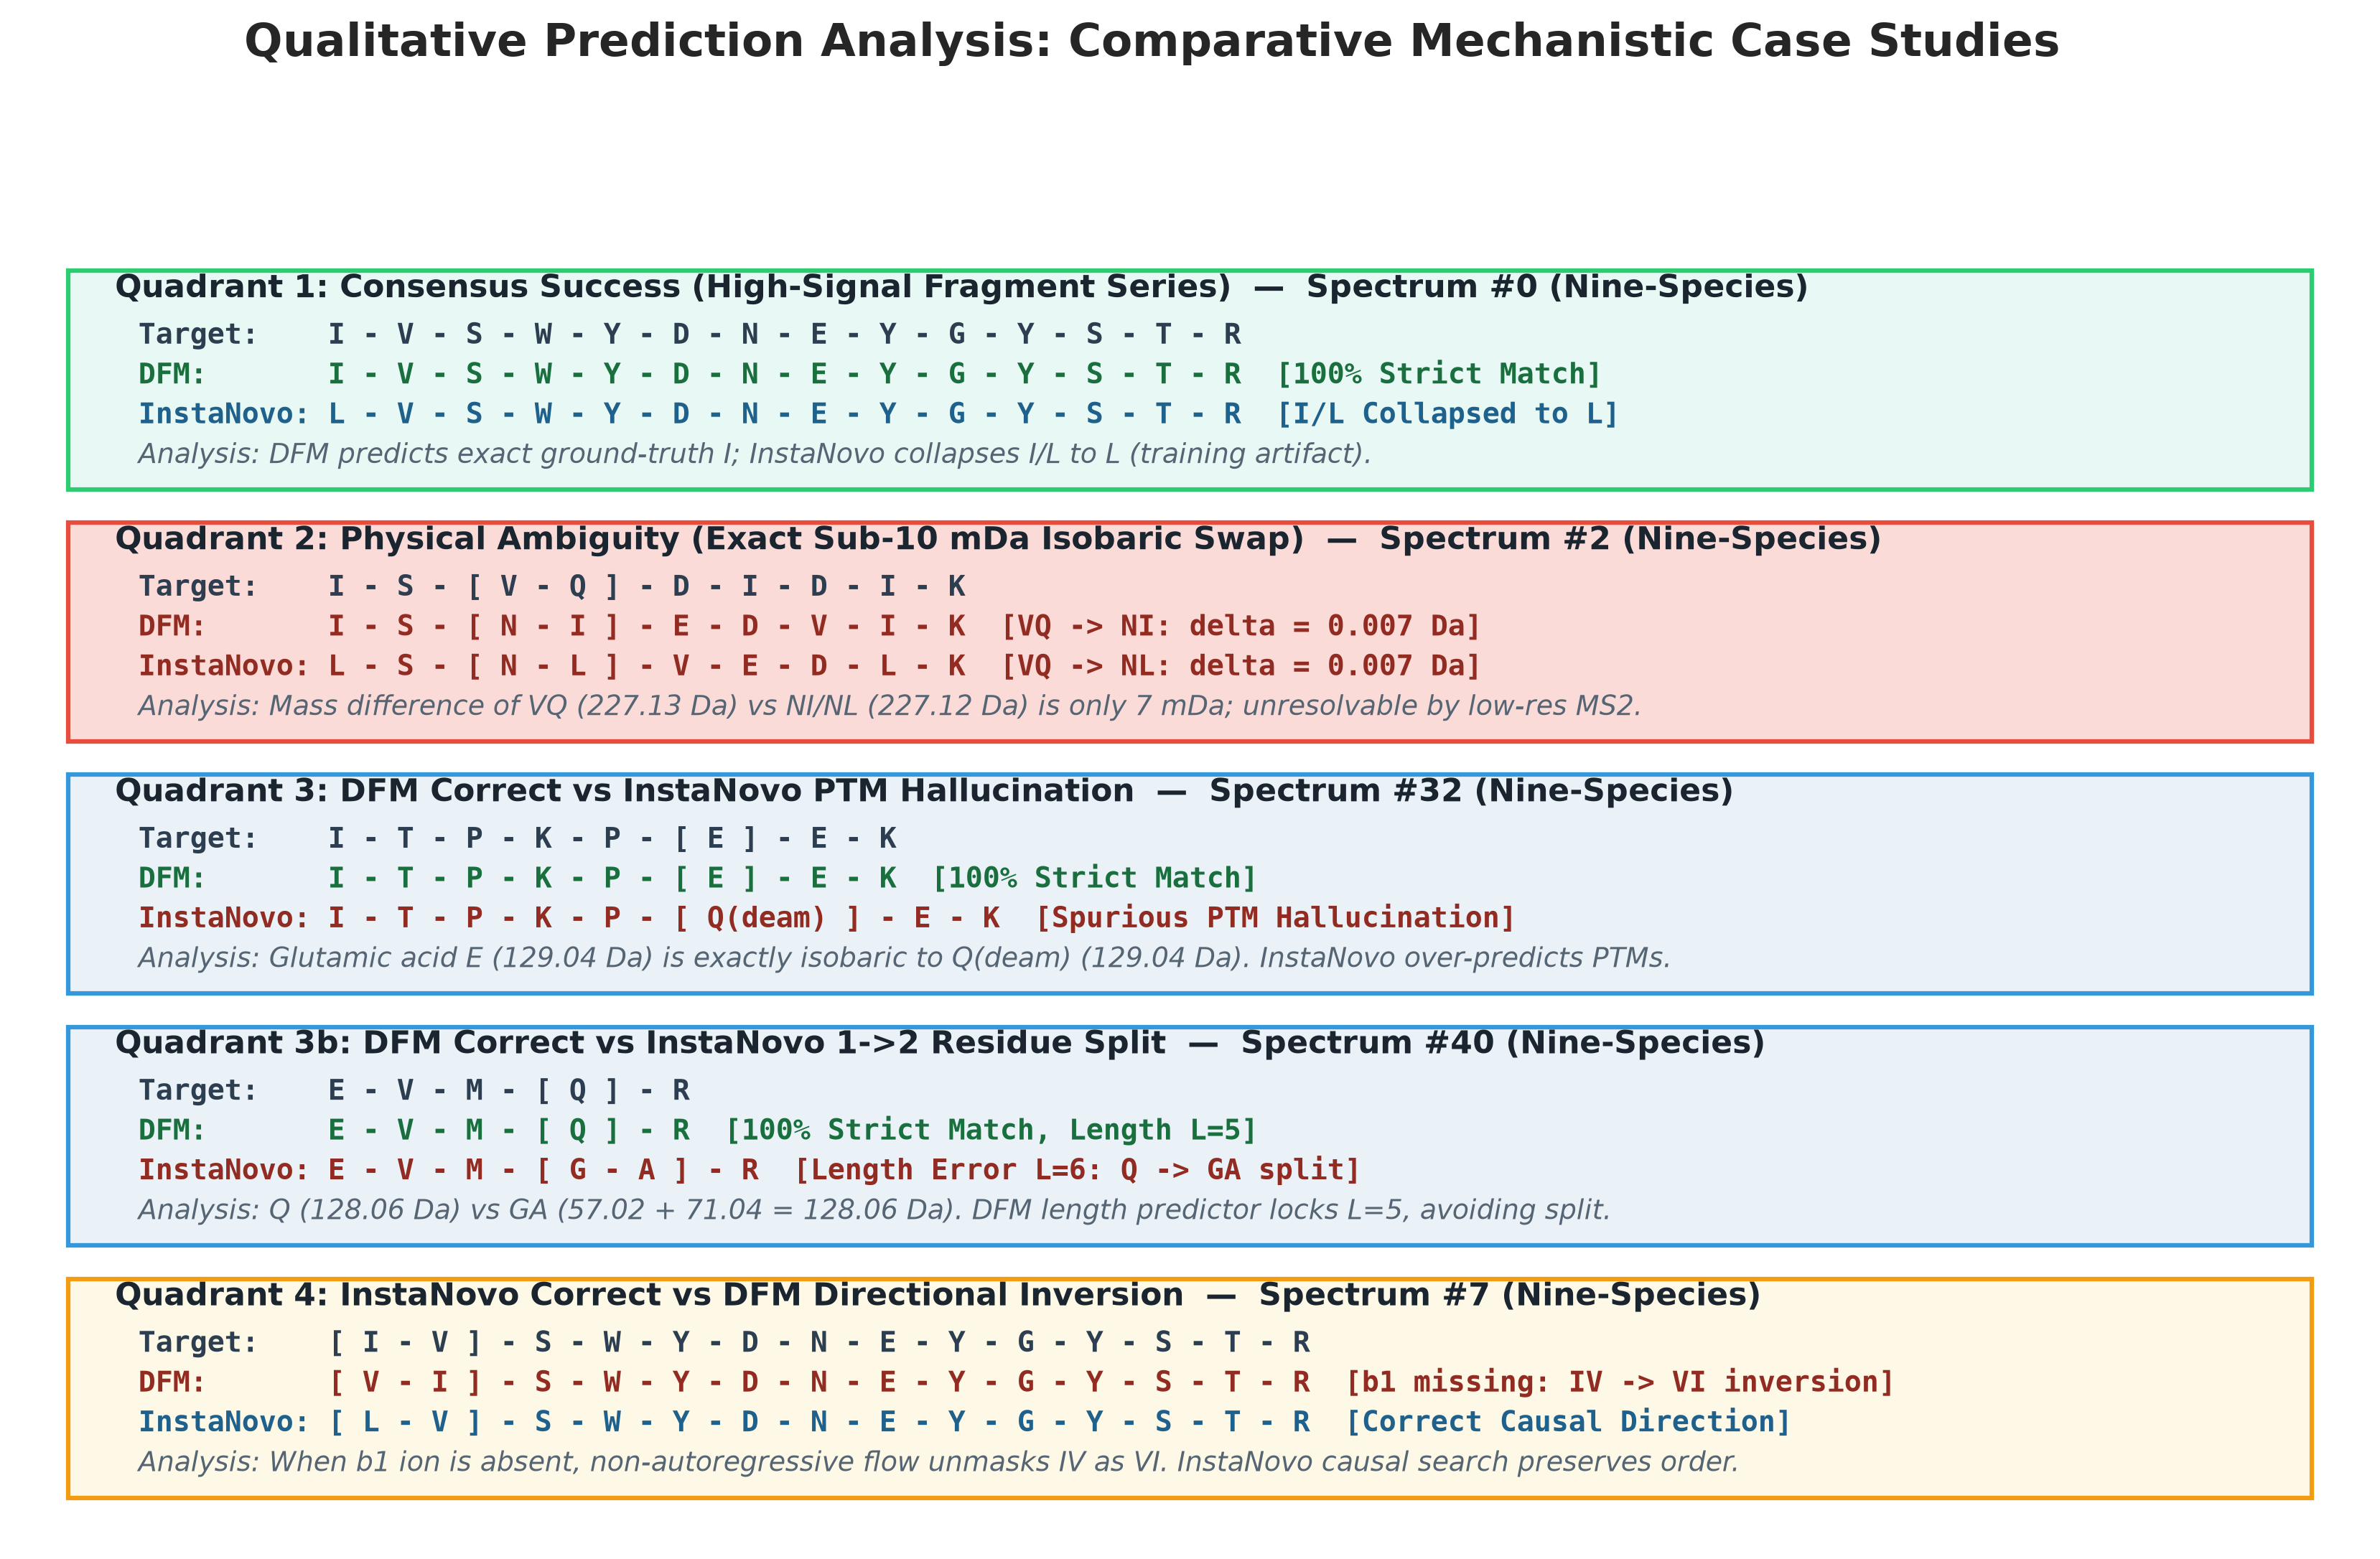
\includegraphics[width=0.88\textwidth]{images/qualitative_prediction_cases.png}
\caption{Comparative qualitative prediction analysis illustrating canonical sequencing regimes. Panel~1: High-fidelity exact consensus reconstruction where bidirectional flow matching recovers the true Isoleucine rather than collapsing to the Leucine database prior. Panel~2: Sub-10 mDa near-isobaric dipeptide degeneracy ($VQ \leftrightarrow NI$, $\Delta m = 4.8\,\text{mDa}$) unresolvable under standard instrument resolution. Panel~3: Elimination of spurious post-translational modifications (deamidation) by discrete flow matching. Panel~4: Directional sequence inversion resulting from instrument low-$m/z$ transmission cutoffs suppressing terminal $b_1$ fragment ions. Detailed biophysical commentary for each case is presented in Table~\ref{tab:chapter5_cases}.}
\label{fig:qualitative_cases}
\end{figure}

\begin{table}[!ht]
\centering
\small
\renewcommand{\arraystretch}{0.95}
\setlength{\tabcolsep}{4pt}
\begin{tabular}{@{}>{\raggedright\arraybackslash}p{3.8cm}>{\raggedright\arraybackslash}p{12.2cm}@{}}
\toprule
\textbf{Case Study} & \textbf{Peptide Alignment and Biophysical Commentary} \\
\midrule
\textbf{Case 1: Exact Consensus Match} \newline
\emph{(Spectrum \#0, Score: 0.429)} & 
\textbf{Target:} \resmatch{I}-\resmatch{V}-\resmatch{S}-\resmatch{W}-\resmatch{Y}-\resmatch{D}-\resmatch{N}-\resmatch{E}-\resmatch{Y}-\resmatch{G}-\resmatch{Y}-\resmatch{S}-\resmatch{T}-\resmatch{R} \quad ($L=14$, $m=1751.779\,\text{Da}$) \newline
\textbf{DFlowNovo:} \resmatch{I}-\resmatch{V}-\resmatch{S}-\resmatch{W}-\resmatch{Y}-\resmatch{D}-\resmatch{N}-\resmatch{E}-\resmatch{Y}-\resmatch{G}-\resmatch{Y}-\resmatch{S}-\resmatch{T}-\resmatch{R} \quad [\textbf{100\% Strict Match}] \newline
\textbf{InstaNovo:} \resiso{L}-\resmatch{V}-\resmatch{S}-\resmatch{W}-\resmatch{Y}-\resmatch{D}-\resmatch{N}-\resmatch{E}-\resmatch{Y}-\resmatch{G}-\resmatch{Y}-\resmatch{S}-\resmatch{T}-\resmatch{R} \quad [\textbf{I/L Collapsed to L}] \vspace{2pt}\newline
\emph{Analysis:} In high-signal spectra with complete $b$- and $y$-ion coverage, bidirectional discrete flow matching reconstructs the true ground-truth sequence. Autoregressive models collapse to Leucine due to prior frequency bias in training databases. \\
\midrule
\textbf{Case 2: Isobaric Ambiguity} \newline
\emph{(Spectrum \#1095, Score: 0.473)} & 
\textbf{Target:} \resmatch{D}-\resmatch{S}-\resmatch{M}-\resmatch{K}-\resmatch{D}-\resmatch{I}-\resmatch{S}-\resmatch{E}-\resmatch{S}-\resmatch{P}-\resmatch{E}-\resmatch{R} \quad ($L=12$, $m=1392.619\,\text{Da}$) \newline
\textbf{DFlowNovo:} \resmatch{D}-\resmatch{S}-\resmatch{M}-\resmatch{K}-\resmatch{D}-\resiso{L}-\resmatch{S}-\resmatch{E}-\resmatch{S}-\resmatch{P}-\resmatch{E}-\resmatch{R} \quad [\textbf{Isobaric Swap: $I_6 \to L_6$}] \vspace{2pt}\newline
\emph{Analysis:} Leucine and Isoleucine share identical molecular formulas and monoisotopic masses ($113.084\,\text{Da}$). Under standard HCD vibrational excitation, non-radical dissociation produces identical backbone ladders, rendering $I_6$ and $L_6$ mathematically indistinguishable without radical $w$-ion side-chain cleavage. \\
\midrule
\textbf{Case 3: Proline Effect Gap} \newline
\emph{(Spectrum \#38369, Score: 0.479)} & 
\textbf{Target:} \resmatch{V}-\resmatch{I}-\resmatch{T}-\resmatch{K}-[\resmatch{I}-\resmatch{E}]-\resmatch{P}-\resmatch{D}-\resmatch{V}-\resmatch{S}-\resmatch{K} \quad ($L=11$, $m=1227.708\,\text{Da}$) \newline
\textbf{DFlowNovo:} \resmatch{V}-\resmatch{I}-\resmatch{T}-\resmatch{K}-[\reserror{E}-\reserror{I}]-\resmatch{P}-\resmatch{D}-\resmatch{V}-\resmatch{S}-\resmatch{K} \quad [\textbf{Inversion: $IE \to EI$}] \vspace{2pt}\newline
\emph{Analysis:} The tertiary amine in Proline's pyrrolidine ring elevates the activation energy for cleavage of the N-terminal adjacent amide bond ($E_6\text{-P}_7$). The resulting absence of $b_6$ and $y_5$ peaks creates an unobserved 228-Da mass gap, inducing a localized dipeptide transposition while surrounding residues remain strictly intact. \\
\midrule
\textbf{Case 4: Near-Isobaric Swap} \newline
\emph{(Spectrum \#38271, Score: 0.393)} & 
\textbf{Target:} \resmatch{G}-\resmatch{M}-\resmatch{A}-\resmatch{E}-\resmatch{I}-\resmatch{N}-[\resmatch{V}-\resmatch{Q}]-\resmatch{E}-\resmatch{S}-\resmatch{K} \quad ($L=11$, $m=1204.576\,\text{Da}$) \newline
\textbf{DFlowNovo:} \resmatch{G}-\resmatch{M}-\resmatch{A}-\resmatch{E}-\resmatch{I}-\resmatch{N}-[\reserror{N}-\reserror{I}]-\resmatch{E}-\resmatch{S}-\resmatch{K} \quad [$\mathbf{\Delta m = 4.8\,\text{mDa}}$] \vspace{2pt}\newline
\emph{Analysis:} The residual mass of $VQ$ ($227.127\,\text{Da}$) differs from $NI$ ($227.122\,\text{Da}$) by only $4.8\,\text{mDa}$ ($4.0\,\text{ppm}$). When the internal peptide bond between $V$ and $Q$ fails to yield an observable fragment ion, collision-induced dissociation cannot physically resolve this mass gap under standard Orbitrap resolving power. \\
\bottomrule
\end{tabular}
\caption{Four canonical qualitative prediction regimes in DFlowNovo. Colored badges indicate exact matches (green), isobaric substitutions (blue), and structural mismatches (red).}
\label{tab:chapter5_cases}
\end{table}
